\begin{figure}[H]
\centering
\resizebox{\columnwidth}{!}{%
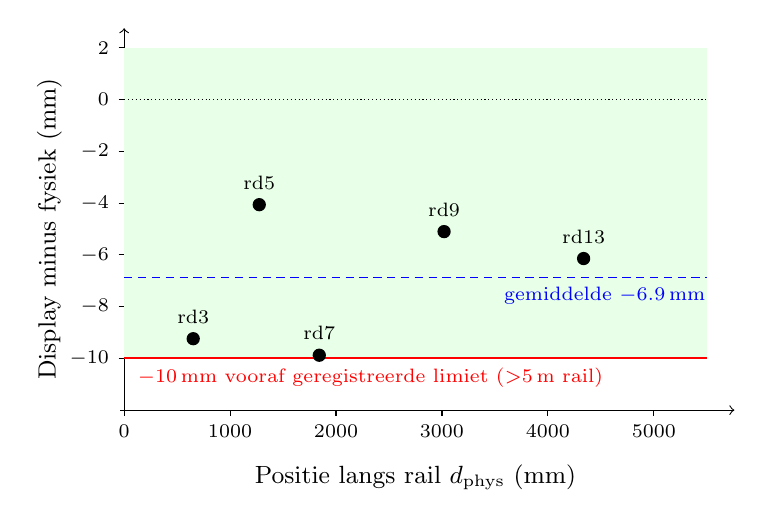
\begin{tikzpicture}
% --- axes ---
\draw[->] (-0.05,0.000) -- (7.75,0.000);
\draw[->] (0,0.000) -- (0,4.85);
% --- threshold / reference lines ---
\fill[green!9] (0,0.657) rectangle (7.40,4.600);  % within-limit (acceptable) zone
\draw[red,thick] (0,0.657) -- (7.40,0.657);
\node[red,font=\scriptsize,below right] at (0.05,0.657) {$-10$\,mm vooraf geregistreerde limiet ($>$5\,m rail)};
\draw[densely dotted] (0,3.943) -- (7.40,3.943);
\draw[blue,densely dashed] (0,1.681) -- (7.40,1.681);
\node[blue,font=\scriptsize,below right] at (4.7,1.681) {gemiddelde $-6.9$\,mm};
% --- y ticks ---
\draw (-0.07,0.657) -- (0,0.657); \node[left,font=\scriptsize] at (-0.07,0.657) {$-10$};
\draw (-0.07,1.314) -- (0,1.314); \node[left,font=\scriptsize] at (-0.07,1.314) {$-8$};
\draw (-0.07,1.971) -- (0,1.971); \node[left,font=\scriptsize] at (-0.07,1.971) {$-6$};
\draw (-0.07,2.629) -- (0,2.629); \node[left,font=\scriptsize] at (-0.07,2.629) {$-4$};
\draw (-0.07,3.286) -- (0,3.286); \node[left,font=\scriptsize] at (-0.07,3.286) {$-2$};
\draw (-0.07,3.943) -- (0,3.943); \node[left,font=\scriptsize] at (-0.07,3.943) {$0$};
\draw (-0.07,4.600) -- (0,4.600); \node[left,font=\scriptsize] at (-0.07,4.600) {$2$};
% --- x ticks ---
\draw (0.000,0.000) -- (0.000,-0.070); \node[below,font=\scriptsize] at (0.000,-0.070) {0};
\draw (1.345,0.000) -- (1.345,-0.070); \node[below,font=\scriptsize] at (1.345,-0.070) {1000};
\draw (2.691,0.000) -- (2.691,-0.070); \node[below,font=\scriptsize] at (2.691,-0.070) {2000};
\draw (4.036,0.000) -- (4.036,-0.070); \node[below,font=\scriptsize] at (4.036,-0.070) {3000};
\draw (5.382,0.000) -- (5.382,-0.070); \node[below,font=\scriptsize] at (5.382,-0.070) {4000};
\draw (6.727,0.000) -- (6.727,-0.070); \node[below,font=\scriptsize] at (6.727,-0.070) {5000};
% --- data points ---
\fill (0.877,0.907) circle (2.4pt);
\node[font=\scriptsize,above=2pt] at (0.877,0.907) {rd3};
\fill (1.716,2.609) circle (2.4pt);
\node[font=\scriptsize,above=2pt] at (1.716,2.609) {rd5};
\fill (2.478,0.697) circle (2.4pt);
\node[font=\scriptsize,above=2pt] at (2.478,0.697) {rd7};
\fill (4.063,2.267) circle (2.4pt);
\node[font=\scriptsize,above=2pt] at (4.063,2.267) {rd9};
\fill (5.835,1.925) circle (2.4pt);
\node[font=\scriptsize,above=2pt] at (5.835,1.925) {rd13};
\node[font=\small] at (3.70,-0.85) {Positie langs rail $d_{\mathrm{phys}}$ (mm)};
\node[font=\small,rotate=90] at (-0.95,2.30) {Display minus fysiek (mm)};
\end{tikzpicture}%
}
\caption{Display-vs-fysiek positiefout bij elke referentiemarker op de 5428\,mm-validatierail (meetronde 2). Elke marker is gerefereerd aan het firmware-encoded begin van zijn rail-part plus een met meetlint gemeten offset binnen dat part (Sectie~\ref{sec:results-validation}). Alle vijf fouten vallen binnen de vooraf geregistreerde $-10$\,mm-tolerantie voor rails langer dan 5\,m en hebben een consistent negatief teken (gemiddelde $-6.9$\,mm), terwijl de pipeline-integratiefout op dezelfde meting vrijwel nul was (Tabel~\ref{tab:validation}); de duiding van dit tekenpatroon staat in Sectie~\ref{sec:conclusion}.}
\label{fig:dv2-error}
\end{figure}
